\documentclass[12pt, a4paper]{article}

\usepackage[utf8]{inputenc}
\usepackage[T1]{fontenc}
\usepackage[spanish]{babel}
\usepackage{amsmath, amssymb}
\usepackage{geometry}
\usepackage{booktabs}
\usepackage{graphicx}
\usepackage{listings}
\usepackage{xcolor}
\usepackage{hyperref}
\usepackage{enumitem}
\usepackage{fancyhdr}
\usepackage{caption}
\usepackage{float}

\geometry{margin=2.5cm}

\definecolor{codeblue}{RGB}{0,102,204}
\definecolor{codegray}{RGB}{100,100,100}

\lstset{
  basicstyle=\ttfamily\small,
  keywordstyle=\color{codeblue}\bfseries,
  commentstyle=\color{codegray}\itshape,
  breaklines=true,
  frame=single,
  numbers=left,
  numberstyle=\tiny\color{codegray},
}

\pagestyle{fancy}
\fancyhead[L]{\small SIA -- TP1: Metodos de Busqueda}
\fancyhead[R]{\small ITBA}
\fancyfoot[C]{\thepage}

\title{
  \textbf{Trabajo Practico 1: Metodos de Busqueda} \\[0.3cm]
  \large Sistemas de Inteligencia Artificial \\[0.2cm]
  \normalsize ITBA -- 2026
}
\author{}
\date{}

\begin{document}

\maketitle
\thispagestyle{empty}
\newpage
\tableofcontents
\newpage

% =============================================================================
\section{Introduccion}
% =============================================================================

Este trabajo practico aborda el estudio de metodos de busqueda en inteligencia artificial a traves de dos ejercicios. El primero es un analisis teorico de heuristicas para una variante del \textbf{8-puzzle con multiples estados objetivo}. El segundo es la implementacion completa de un solver de \textbf{Sokoban} usando los algoritmos BFS, DFS, Greedy y A*, con al menos dos heuristicas admisibles.

El codigo fuente, instrucciones de ejecucion y niveles de prueba se encuentran en el repositorio del proyecto. Para ejecutar el solver:

\begin{lstlisting}[language=bash, numbers=none]
python3 -m src.main --iterations 10 --seed 42
\end{lstlisting}

% =============================================================================
\section{Parte 1: Heuristicas para el 8-puzzle}
% =============================================================================

\subsection{Planteo del problema}

Se trabaja con una variante del 8-puzzle en la que la condicion de solucion no es una disposicion fija, sino que las fichas deben cumplir \textbf{restricciones de adyacencia}. Cada ficha numerada del 1 al 8 debe ser vecina (horizontal o vertical) de ciertos numeros especificos. El grafo de adyacencia requerido es:

\begin{center}
\small
\begin{tabular}{cl}
\toprule
\textbf{Ficha} & \textbf{Adyacentes requeridos} \\
\midrule
1 & 2, 4 \\
2 & 1, 3, 5 \\
3 & 2, 6 \\
4 & 1, 5, 7 \\
5 & 2, 4, 6, 8 \\
6 & 3, 5, 9 \\
7 & 4, 8 \\
8 & 5, 7, 9 \\
\bottomrule
\end{tabular}
\end{center}

\subsection{Estructura de estado}

Un estado se define por las posiciones de las 9 fichas (1--8 mas el vacio) en el tablero $3 \times 3$. Se puede representar como un arreglo 1D de 9 elementos. Las acciones posibles son mover el espacio vacio a una casilla adyacente (arriba, abajo, izquierda, derecha), respetando los limites del tablero.

\subsection{Observacion clave: la ficha 5 va al centro}

En el grafo de adyacencias, la ficha \textbf{5} tiene grado 4 (es adyacente a 2, 4, 6 y 8). En un tablero $3 \times 3$, la unica casilla con 4 vecinos es el \textbf{centro}. Por lo tanto, en toda solucion valida, el 5 debe estar en la casilla central. Esto genera multiples estados meta posibles (rotaciones y reflexiones). Llamamos $G$ al conjunto de todos los estados solucion.

\subsection{Heuristica 1: $h_5$ -- distancia del 5 al centro}

Definimos una heuristica por casos basada en la posicion del 5 y del vacio:

$$
h_5(s) = \begin{cases}
d_M(\square, 5) - 1 & \text{si 5 en esquina y vacio no adyacente a 5} \\
d_M(5, c) & \text{si 5 en esquina y vacio adyacente a 5} \\
d_M(\square, c) & \text{si 5 en borde y vacio no en centro} \\
d_M(5, c) & \text{si 5 en borde y vacio en centro} \\
0 & \text{si 5 ya en centro}
\end{cases}
$$

donde $d_M$ denota distancia Manhattan, $\square$ es el vacio y $c$ es la casilla central.

\textbf{Admisibilidad:} En cada caso, $h_5$ mide una condicion necesaria antes de alcanzar cualquier solucion. Caso 1: antes de mover al 5, el vacio debe llegar adyacente a el ($\geq k-1$ movimientos). Caso 2: la distancia Manhattan del 5 al centro requiere al menos esa cantidad de movimientos del 5. Caso 3: el vacio debe pasar por el centro. Caso 4: falta al menos 1 movimiento del 5. Caso 5: ya cumplido. En todos los casos $h_5(s) \leq h^*(s)$.

\subsection{Heuristica 2: $h_G$ -- Manhattan minima sobre todos los goals}

$$h_G(s) = \min_{g \in G} \sum_{i=1}^{8} d_M(\text{pos}_s(i), \text{pos}_g(i))$$

donde $G$ es el conjunto de estados solucion validos y la suma recorre fichas 1 a 8 (excluyendo el vacio).

\textbf{Admisibilidad:} Para un goal fijo $g$, la suma Manhattan es admisible: cada movimiento desplaza una sola ficha una casilla, asi que la suma decrece a lo sumo en 1 por jugada. Como esto vale para cada $g \in G$, el minimo tambien es admisible.

\subsection{Combinacion}

$$h(s) = \max\big(h_5(s),\; h_G(s)\big)$$

El maximo de dos heuristicas admisibles es admisible: $\max(h_1, h_2) \leq \max(h^*, h^*) = h^*$. Se usa $\max$ y no suma porque la suma podria doble-contar esfuerzo, rompiendo admisibilidad. La combinacion aprovecha la informacion estructural de $h_5$ (centrar el 5) y la informacion global de $h_G$ (ordenar todas las fichas).

\subsection{Metodos de busqueda recomendados}

\begin{itemize}
  \item \textbf{A*} con $h = \max(h_5, h_G)$: optimo (heuristicas admisibles) y eficiente.
  \item \textbf{Greedy} con $h$: rapido pero sin garantia de optimalidad.
  \item \textbf{BFS}: optimo con costos unitarios pero explora mas estados.
  \item \textbf{DFS}: encuentra alguna solucion, sin garantia de optimalidad.
\end{itemize}

% =============================================================================
\section{Parte 2: Sokoban}
% =============================================================================

\subsection{Descripcion del problema}

Sokoban es un puzzle donde un jugador empuja cajas hasta posiciones objetivo dentro de un tablero con paredes. Las reglas: el jugador se mueve en 4 direcciones, las cajas solo se empujan (no se tiran), solo una caja a la vez, y el puzzle se resuelve cuando todas las cajas estan sobre todos los goals.

\subsection{Representacion del estado}

Cada estado se modela con la clase \texttt{SokobanState}:

\begin{itemize}
  \item \textbf{Posicion del jugador}: tupla $(fila, columna)$.
  \item \textbf{Posiciones de las cajas}: \texttt{frozenset} de posiciones (inmutable y hasheable).
  \item \textbf{Layout estatico}: \texttt{BoardLayout} compartido entre estados (paredes, goals, piso).
\end{itemize}

La condicion de goal es: $\texttt{boxes} = \texttt{goals}$ (igualdad de conjuntos).

Cada accion (movimiento del jugador) tiene costo 1, independientemente de si empuja una caja o no. La identidad de un estado para el conjunto de explorados esta dada por $(jugador, cajas)$.

% =============================================================================
\section{Algoritmos de busqueda implementados}
% =============================================================================

\begin{center}
\begin{tabular}{lllcc}
\toprule
\textbf{Algoritmo} & \textbf{Tipo} & \textbf{Estructura} & \textbf{Optimo} & \textbf{Completo} \\
\midrule
BFS & Desinformado & Cola FIFO & Si & Si \\
DFS & Desinformado & Pila LIFO & No & No \\
Greedy & Informado & Min-heap por $h$ & No & No \\
A* & Informado & Min-heap por $g+h$ & Si (h admisible) & Si \\
\bottomrule
\end{tabular}
\end{center}

\textbf{Detalle de implementacion de A*:} La implementacion usa graph search con reapertura de nodos cerrados. Cuando A* encuentra un camino mas barato a un estado ya expandido, lo reabre y re-expande. Esto garantiza optimalidad con heuristicas admisibles (no requiere consistencia). Se usa un diccionario \texttt{best\_g} para trackear el mejor costo conocido por estado, y \texttt{closed\_g} para los expandidos. Si un sucesor tiene menor costo que \texttt{best\_g}, se actualiza y se reinserta en el heap.

El tie-breaking en el heap usa la tupla $(f, h, -g, secuencia)$: ante igual $f$, prefiere menor $h$ (mas cercano al goal); ante igual $h$, prefiere mayor $g$ (mas profundo).

% =============================================================================
\section{Heuristicas implementadas}
% =============================================================================

\subsection{Heuristica 1: Deadlocks estaticos ($h_{\text{deadlock}}$)}

Detecta posiciones donde una caja \textbf{nunca puede llegar a ningun goal}, usando un modelo relajado de una sola caja sin obstaculos.

\textbf{Algoritmo:} BFS inverso desde los goals. Para cada posicion, se evalua desde donde podria haber llegado una caja con un empuje valido (la posicion previa de la caja y la posicion de soporte del jugador deben ser piso). Las posiciones no alcanzadas son \textbf{prohibidas}.

$$h_{\text{deadlock}}(s) = \begin{cases} +\infty & \text{si alguna caja (fuera de goal) esta en posicion prohibida} \\ 0 & \text{caso contrario} \end{cases}$$

\textbf{Admisibilidad:} Si devuelve $\infty$, el estado es irrecuperable (costo real tambien infinito). Si devuelve 0, nunca sobreestima. El analisis se precomputa una vez por layout y se cachea con \texttt{@lru\_cache}.

\subsection{Heuristica 2: Minimum matching ($h_{\text{match}}$)}

Calcula la asignacion optima de cajas no colocadas a goals no ocupados, minimizando la suma de distancias Manhattan.

$$h_{\text{match}}(s) = \min_{\sigma} \sum_{i} d_M(\text{caja}_i, \text{goal}_{\sigma(i)})$$

donde las cajas son $B = \texttt{boxes} - \texttt{goals}$ (no colocadas) y los goals son $G' = \texttt{goals} - \texttt{boxes}$ (no ocupados).

Se resuelve con el \textbf{algoritmo Hungaro} via \texttt{scipy.optimize.linear\_sum\_assignment} en $O(n^3)$. Optimizaciones: shortcircuit para 0 cajas (retorna 0) y para 1 caja (retorna Manhattan directo sin numpy).

\textbf{Admisibilidad:} Manhattan es lower bound del costo real de empujar una caja (ignora paredes y otras cajas). El matching minimo no doble-cuenta porque asigna cada goal a una sola caja.

\subsection{Heuristica combinada ($h_{\text{combined}}$)}

$$h_{\text{combined}}(s) = \max\big(h_{\text{match}}(s),\; h_{\text{deadlock}}(s)\big)$$

\textbf{Admisibilidad:} El maximo de dos heuristicas admisibles es admisible. En la practica, $h_{\text{deadlock}}$ aporta poda de estados imposibles y $h_{\text{match}}$ aporta guia numerica.

% =============================================================================
\section{Resultados experimentales}
% =============================================================================

Se ejecutaron los 8 metodos (BFS, DFS, Greedy$\times$3 heuristicas, A*$\times$3 heuristicas) sobre 4 niveles con 10 iteraciones cada uno (seed=42). Las metricas reportadas son: resultado (exito/fracaso), costo de la solucion, nodos expandidos, nodos en frontera al finalizar, y tiempo de procesamiento.

Todos los metodos resolvieron todos los niveles ($\text{success\_rate} = 1.0$).

\subsection{Costo por nivel}

\begin{figure}[H]
\centering
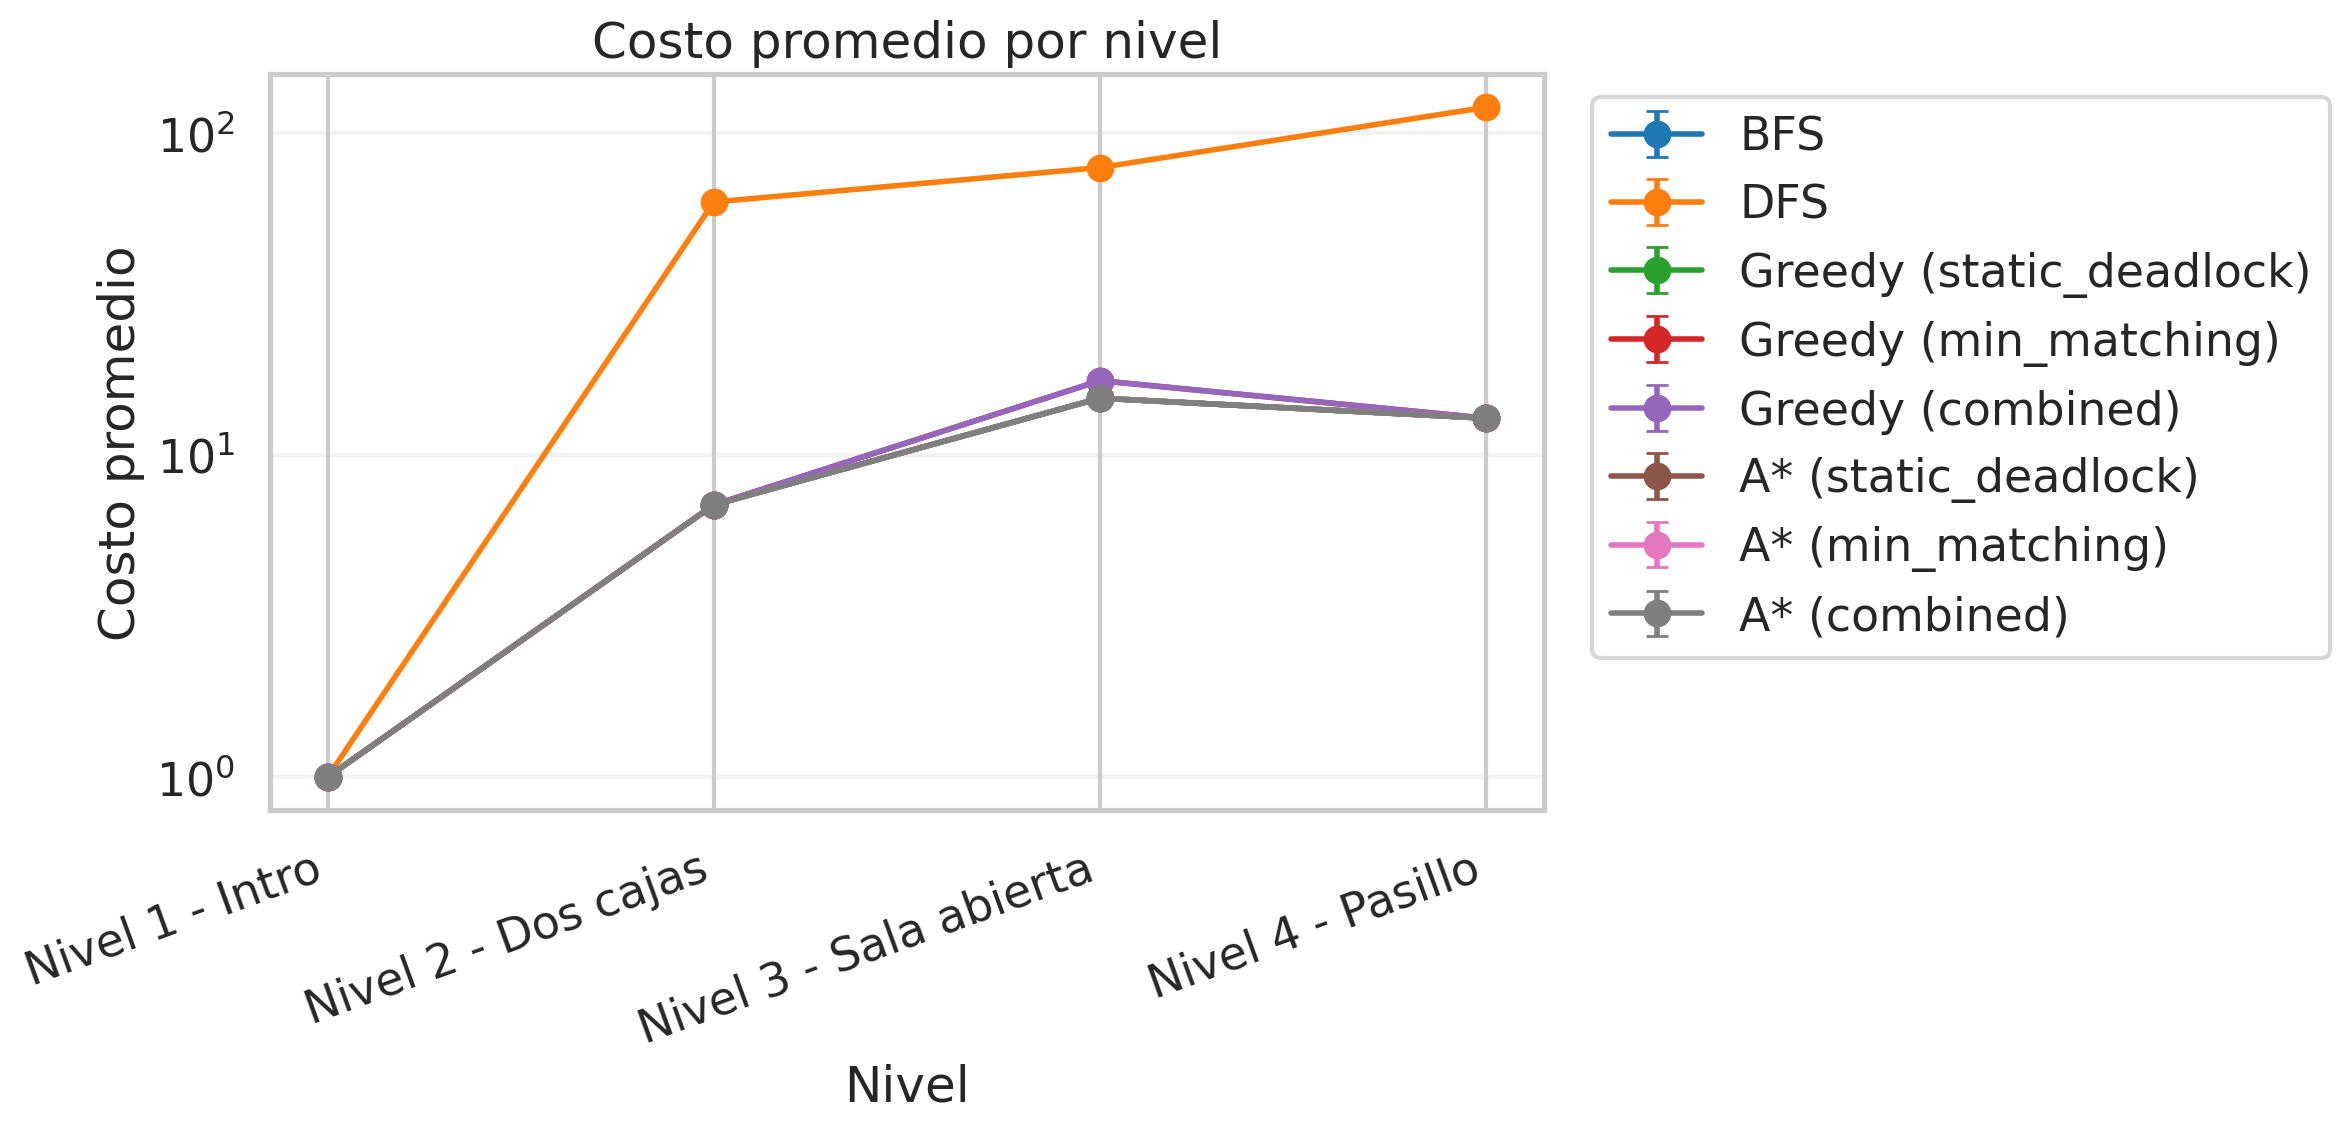
\includegraphics[width=0.85\textwidth]{../results/plots/cost_by_level_errorbars.png}
\caption{Costo promedio por nivel. BFS y A* (todos los variantes) encuentran la solucion optima. DFS encuentra soluciones significativamente mas largas. Greedy con min\_matching/combined empata el optimo en estos niveles.}
\end{figure}

\begin{center}
\small
\begin{tabular}{lrrrr}
\toprule
\textbf{Metodo} & \textbf{Nivel 1} & \textbf{Nivel 2} & \textbf{Nivel 3} & \textbf{Nivel 4} \\
\midrule
BFS & 1 & 7 & 15 & 13 \\
DFS & 1 & 61 & 78 & 120 \\
Greedy (min\_matching) & 1 & 7 & 17 & 13 \\
Greedy (static\_deadlock) & 1 & 7 & 15 & 13 \\
A* (combined) & 1 & 7 & 15 & 13 \\
A* (min\_matching) & 1 & 7 & 15 & 13 \\
A* (static\_deadlock) & 1 & 7 & 15 & 13 \\
\bottomrule
\end{tabular}
\end{center}

DFS encuentra soluciones de costo 61, 78 y 120 donde el optimo es 7, 15 y 13 respectivamente. Esto demuestra que DFS no garantiza optimalidad.

\subsection{Algoritmos optimos: tiempo, nodos y frontera}

\begin{figure}[H]
\centering
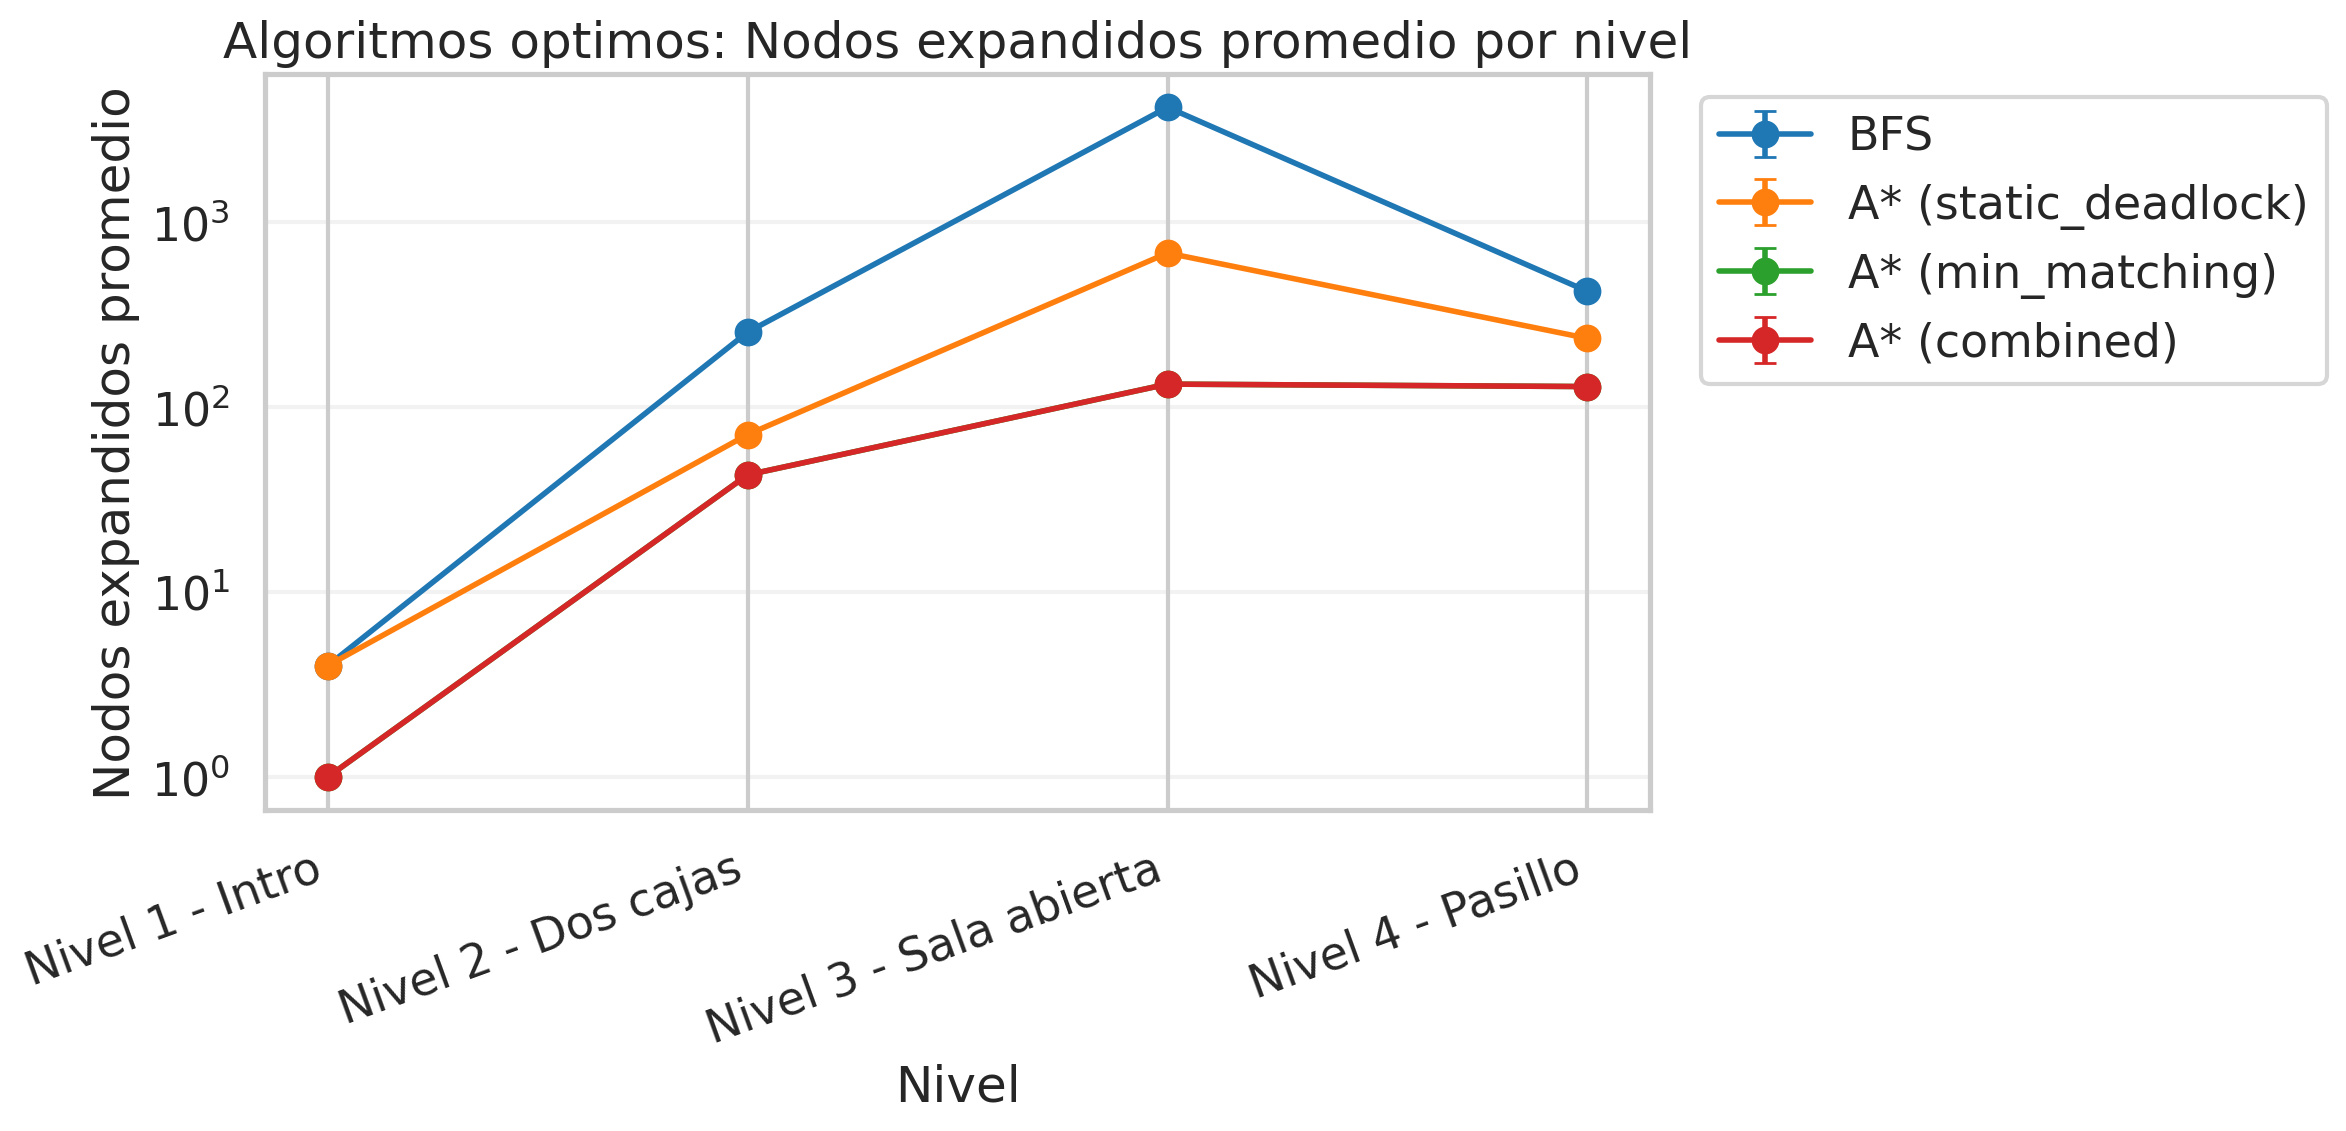
\includegraphics[width=0.85\textwidth]{../results/plots/optimal_nodes_expanded_by_level.png}
\caption{Nodos expandidos por los algoritmos optimos. BFS explora significativamente mas que A*. A*(combined) y A*(min\_matching) coinciden porque min\_matching es consistente y no requiere reapertura.}
\end{figure}

\begin{figure}[H]
\centering
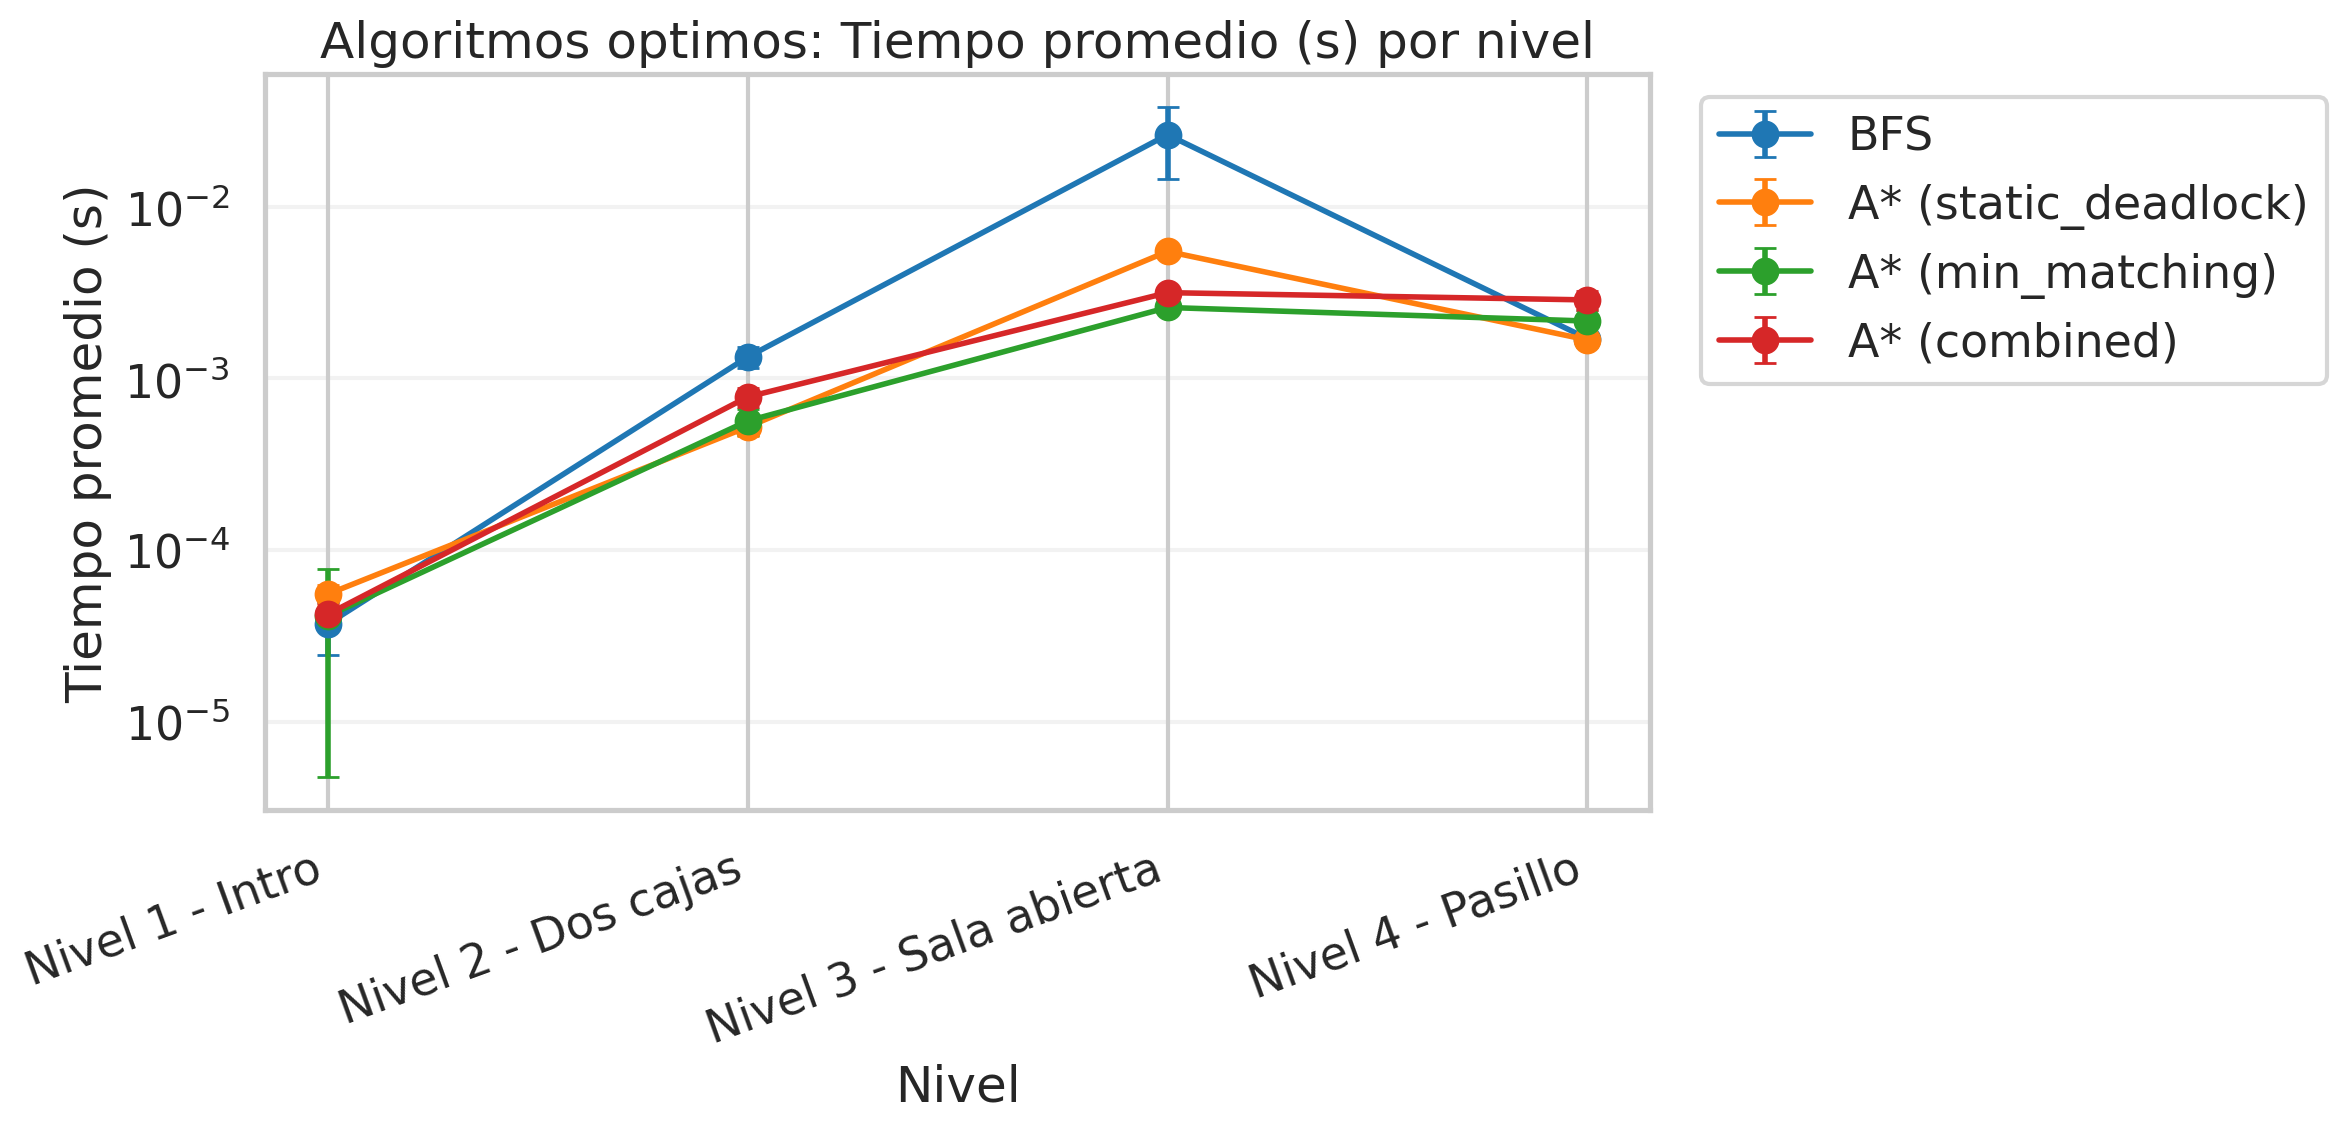
\includegraphics[width=0.85\textwidth]{../results/plots/optimal_time_by_level.png}
\caption{Tiempo de ejecucion de los algoritmos optimos. Escala logaritmica. A* reduce el tiempo respecto de BFS en los niveles con mayor branching (Nivel 3).}
\end{figure}

\begin{figure}[H]
\centering
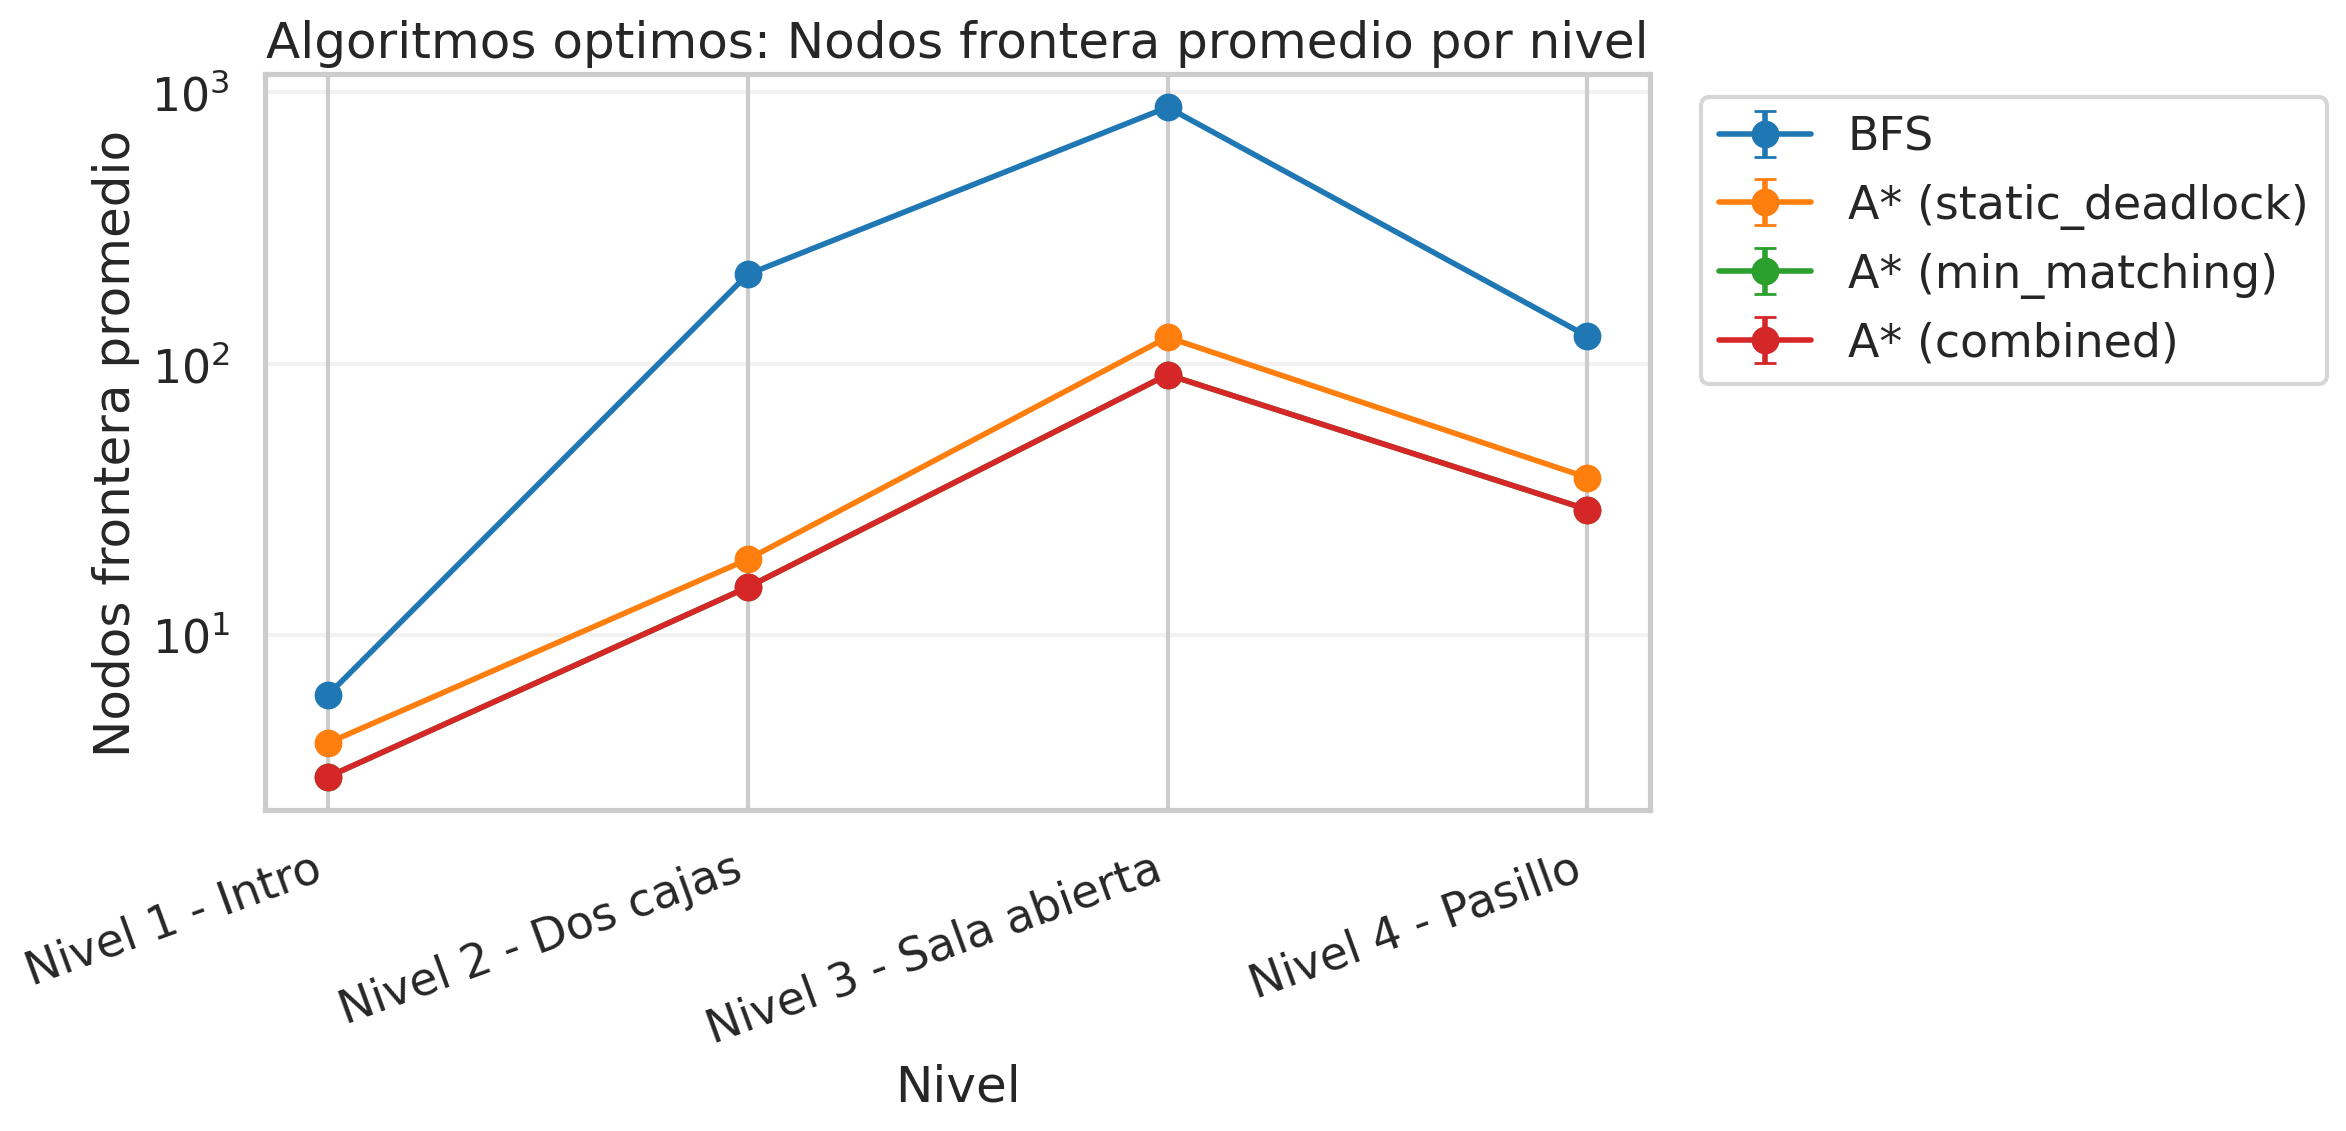
\includegraphics[width=0.85\textwidth]{../results/plots/optimal_frontier_count_by_level.png}
\caption{Nodos en frontera al finalizar. A*(combined) mantiene la frontera mas chica. Nota: esta metrica es la frontera al terminar, no el pico de memoria.}
\end{figure}

\begin{center}
\small
\begin{tabular}{lrrrr}
\toprule
\textbf{Nodos expandidos} & \textbf{Nivel 1} & \textbf{Nivel 2} & \textbf{Nivel 3} & \textbf{Nivel 4} \\
\midrule
BFS & 4 & 254 & 4171 & 422 \\
A* (static\_deadlock) & 4 & 71 & 680 & 235 \\
A* (min\_matching) & 1 & 43 & 133 & 129 \\
A* (combined) & 1 & 43 & 133 & 129 \\
\bottomrule
\end{tabular}
\end{center}

A*(combined) expande 31$\times$ menos nodos que BFS en Nivel 3 (133 vs 4171). A*(static\_deadlock) queda intermedio porque $h=0$ para la mayoria de estados (no guia la busqueda, solo poda deadlocks).

\subsection{Algoritmos no optimos: DFS y Greedy}

\begin{figure}[H]
\centering
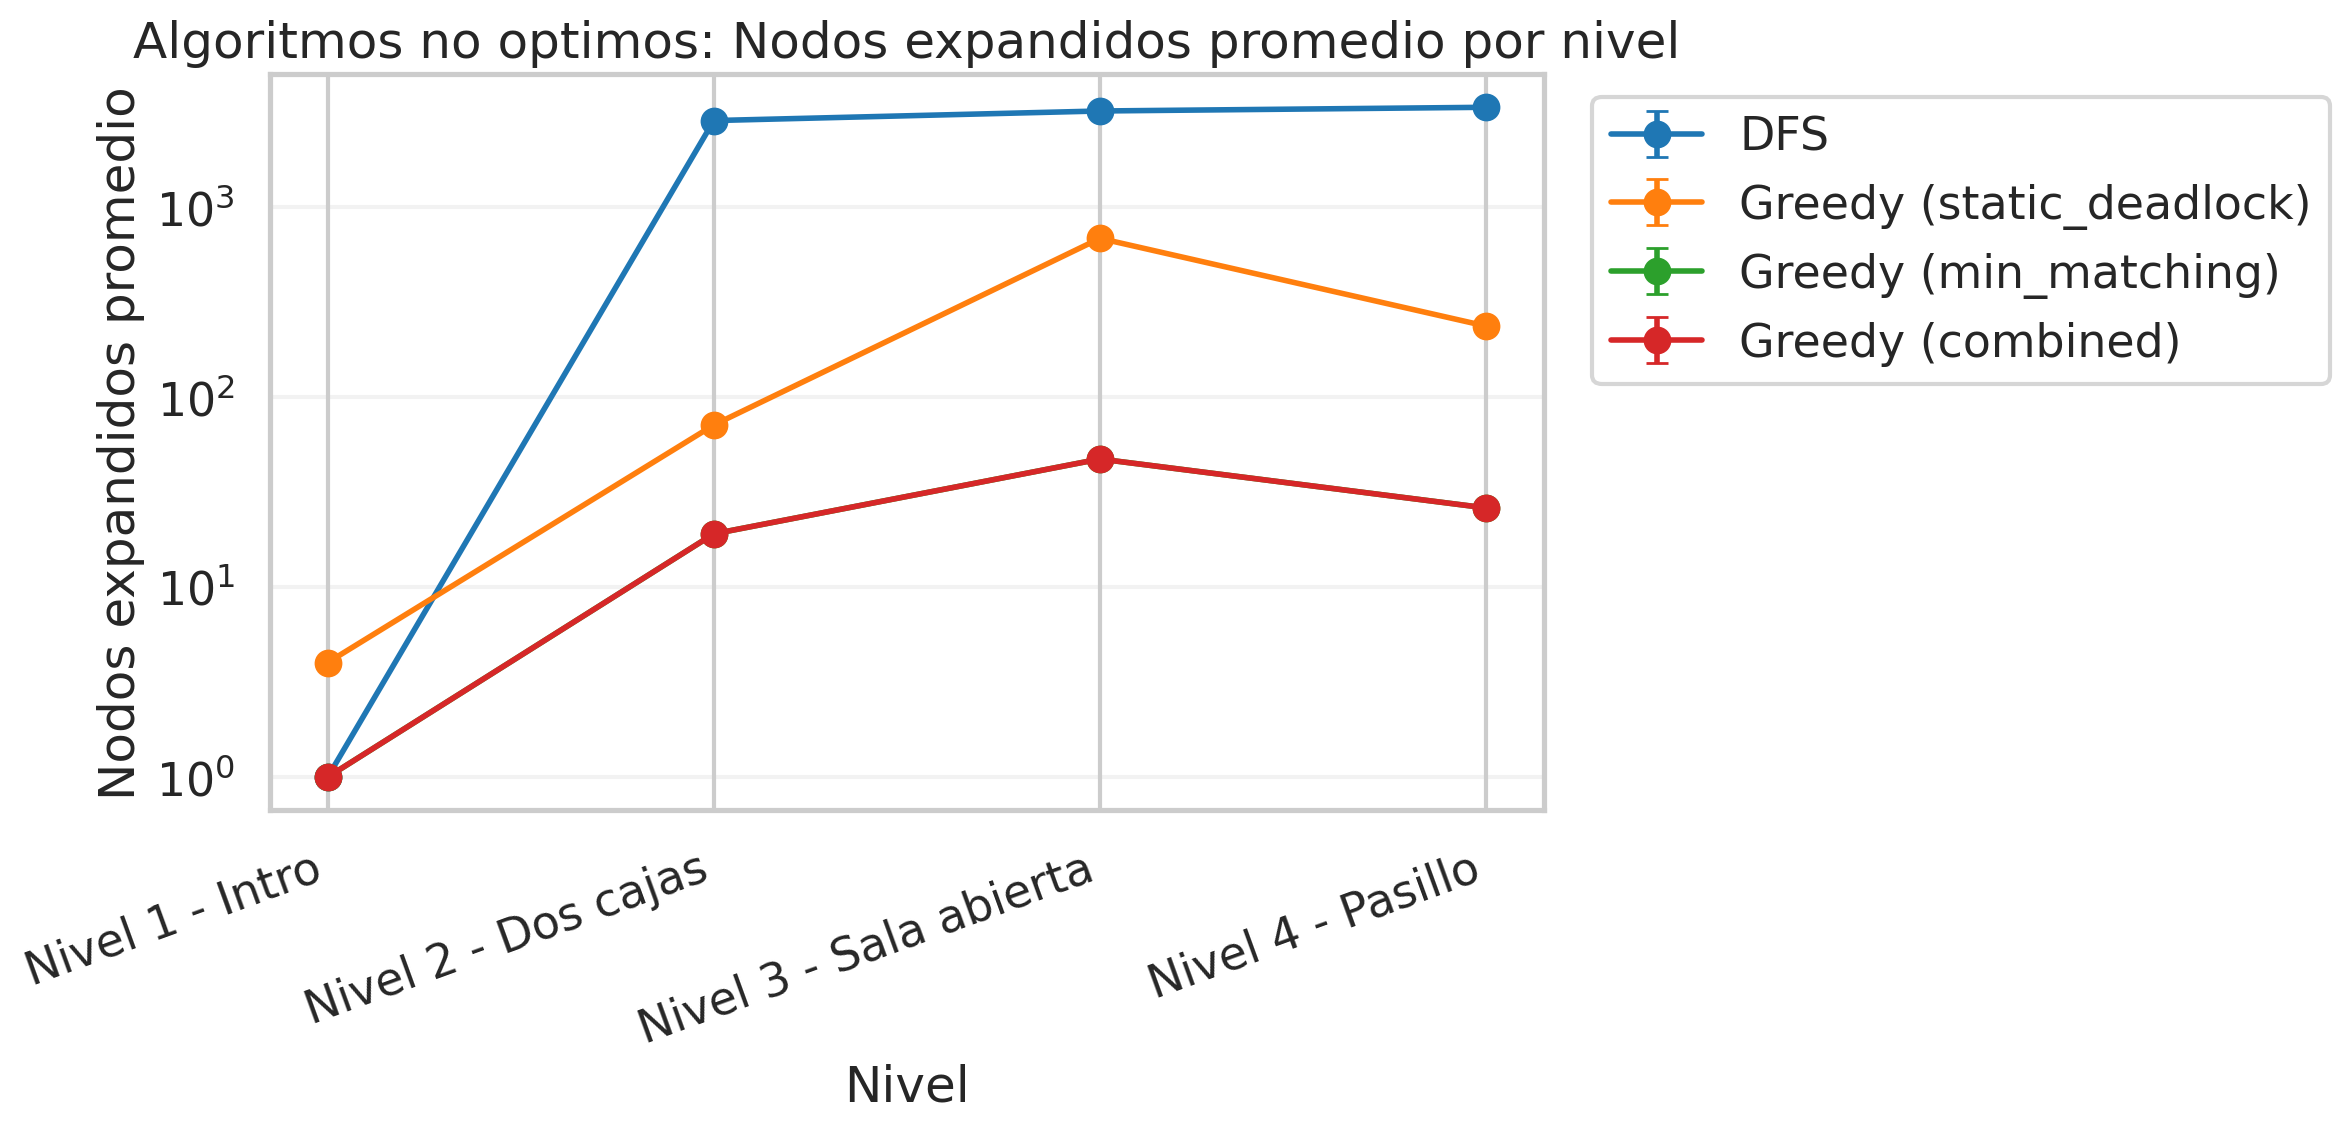
\includegraphics[width=0.85\textwidth]{../results/plots/non_optimal_nodes_expanded_by_level.png}
\caption{Nodos expandidos por DFS y las variantes de Greedy. DFS domina con miles de nodos. Greedy con min\_matching o combined expande menos de 50 nodos.}
\end{figure}

\begin{figure}[H]
\centering
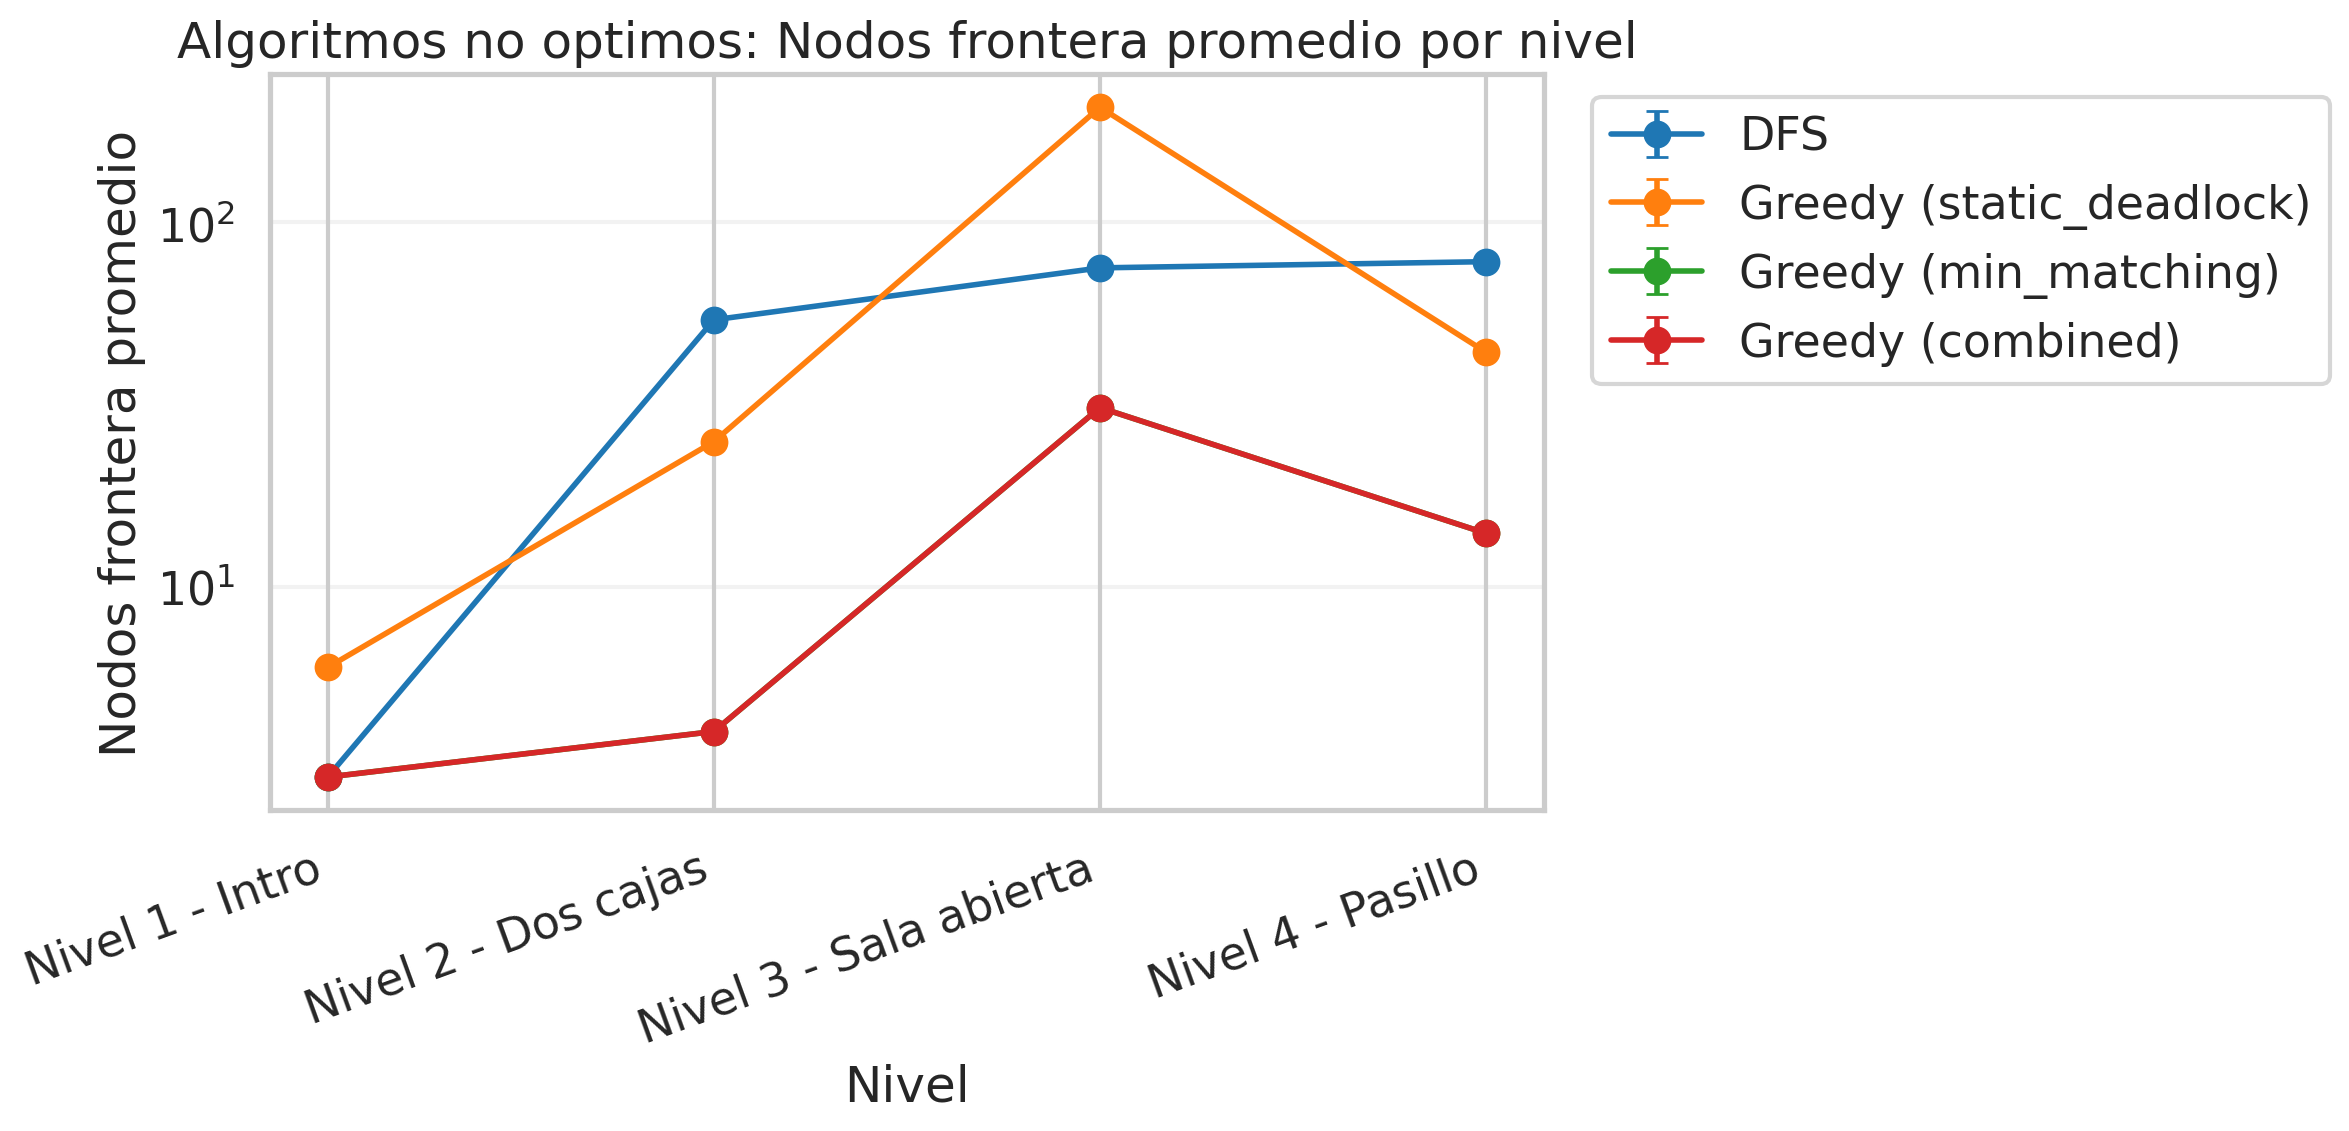
\includegraphics[width=0.85\textwidth]{../results/plots/non_optimal_frontier_count_by_level.png}
\caption{Frontera de los algoritmos no optimos. Greedy(static\_deadlock) acumula frontera comparable a DFS porque $h=0$ no guia la busqueda.}
\end{figure}

\subsection{Comparativas directas}

\begin{figure}[H]
\centering
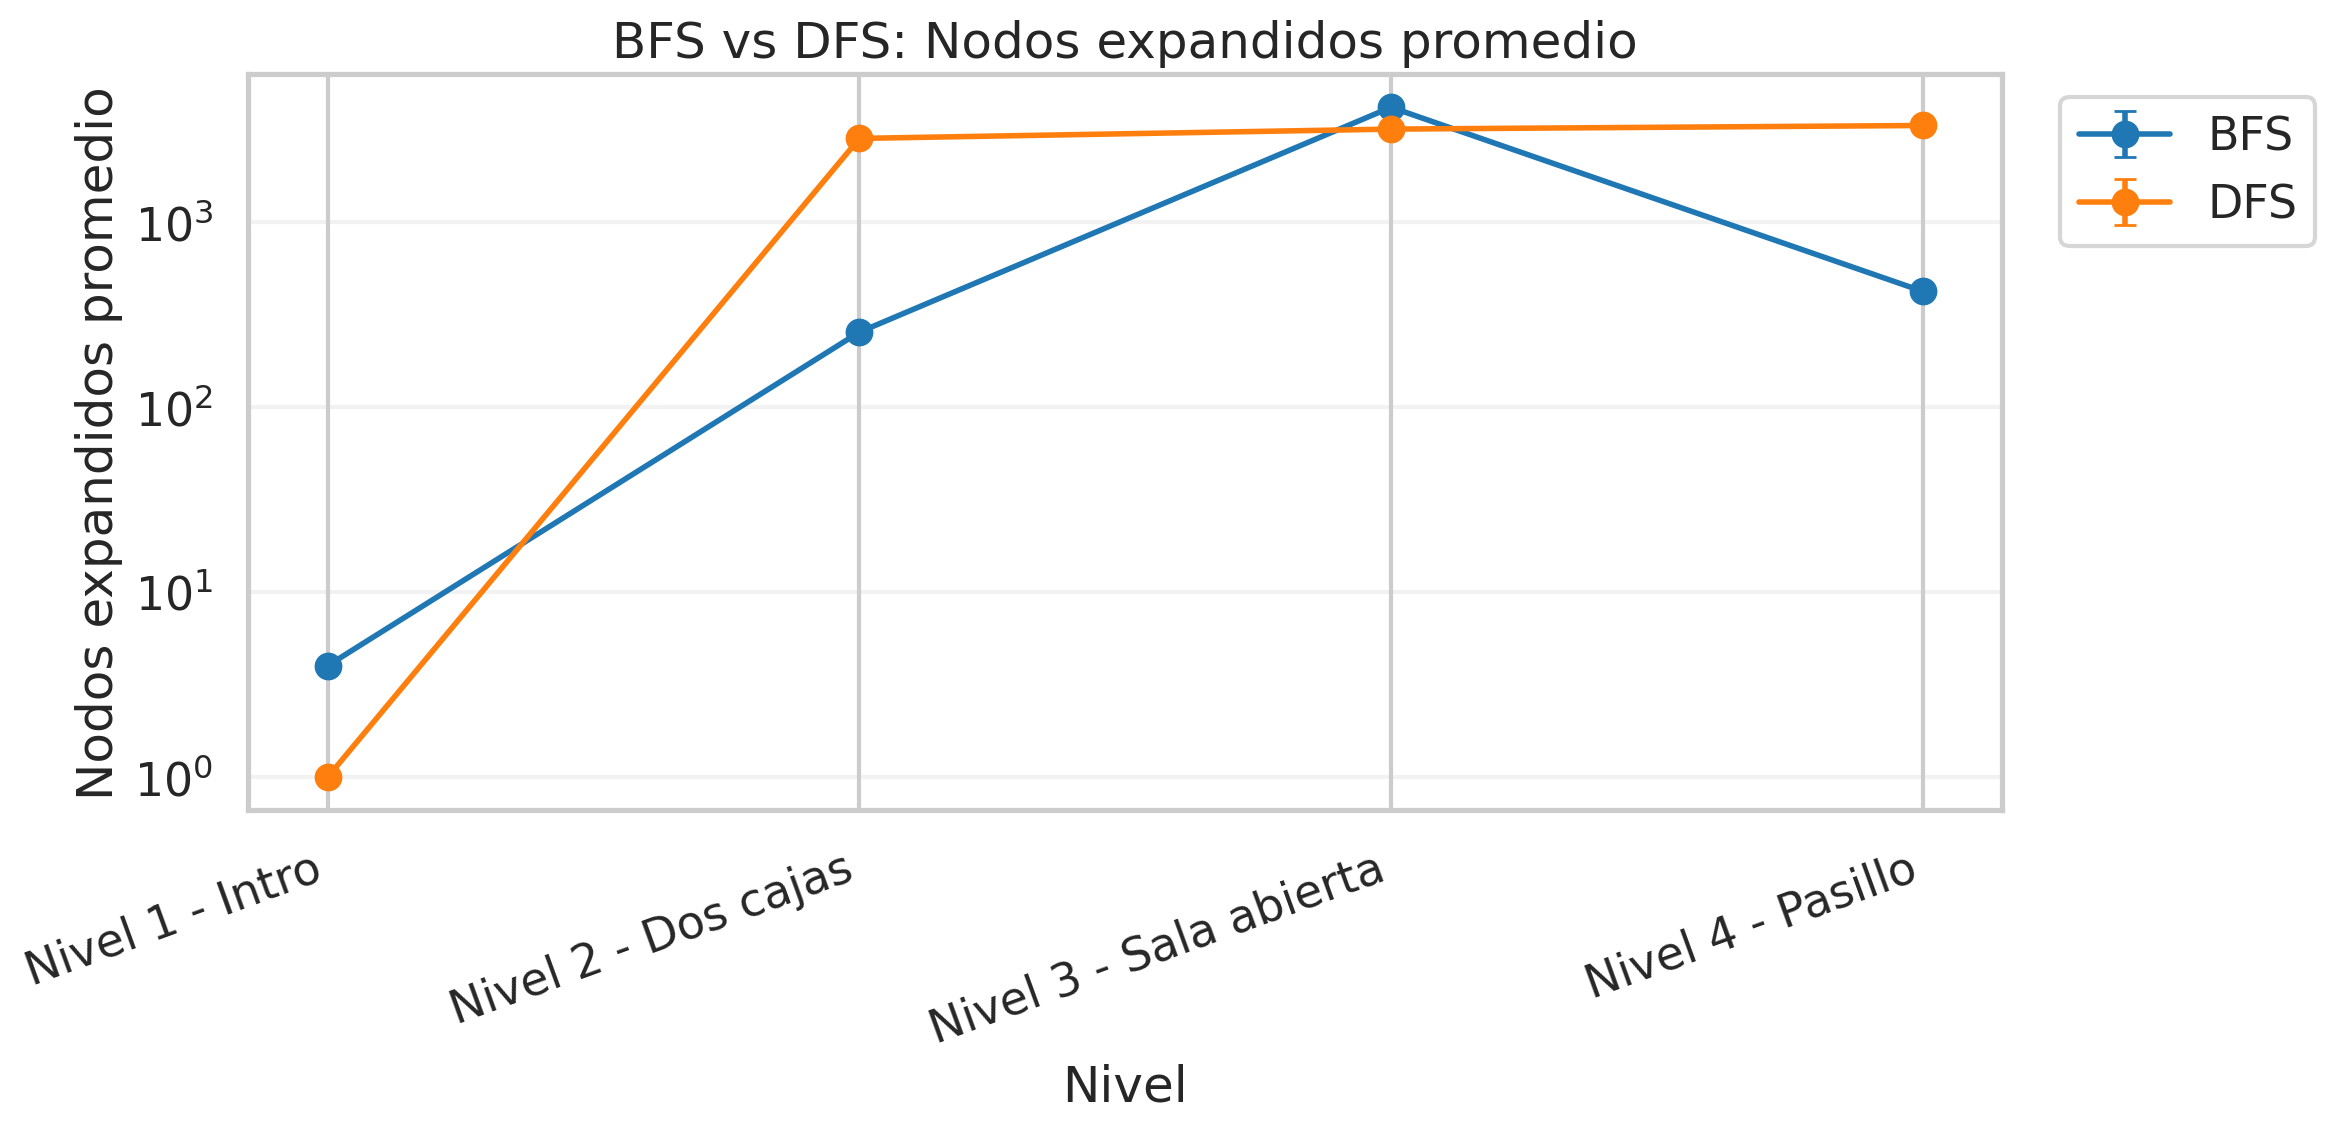
\includegraphics[width=0.85\textwidth]{../results/plots/bfs_vs_dfs_nodes_expanded_errorbars.png}
\caption{BFS vs DFS: nodos expandidos. DFS expande mas nodos en todos los niveles excepto Nivel 3 donde se acercan.}
\end{figure}

\begin{figure}[H]
\centering
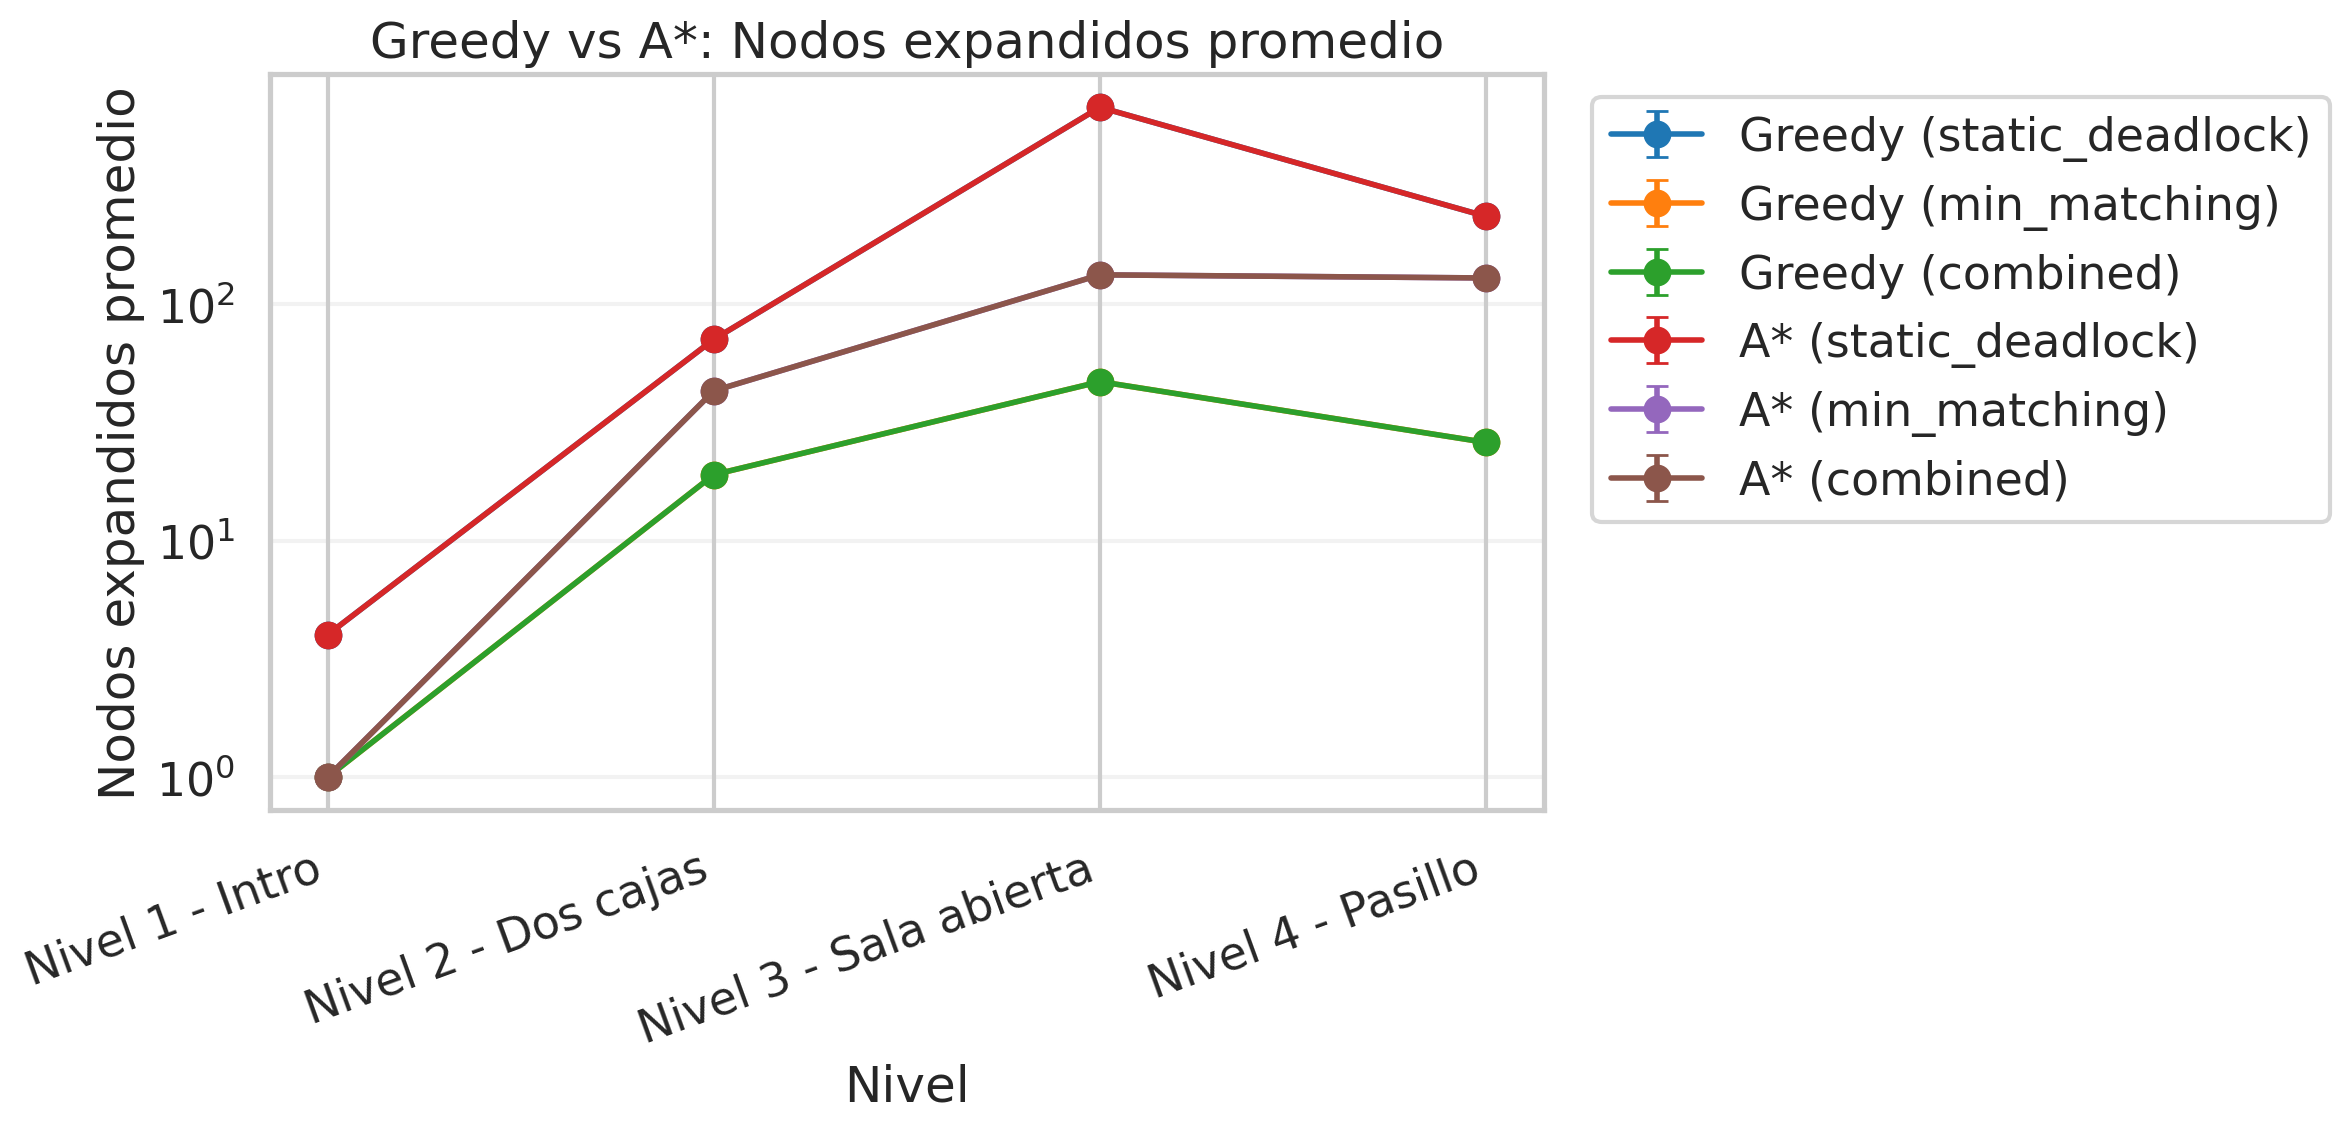
\includegraphics[width=0.85\textwidth]{../results/plots/greedy_vs_astar_nodes_expanded_errorbars.png}
\caption{Greedy vs A*: nodos expandidos. Greedy expande menos nodos (no busca optimalidad) pero A* garantiza costo optimo. A*(static\_deadlock) expande mucho mas porque $h=0$ no guia.}
\end{figure}

\subsection{Distribucion de costo}

\begin{figure}[H]
\centering
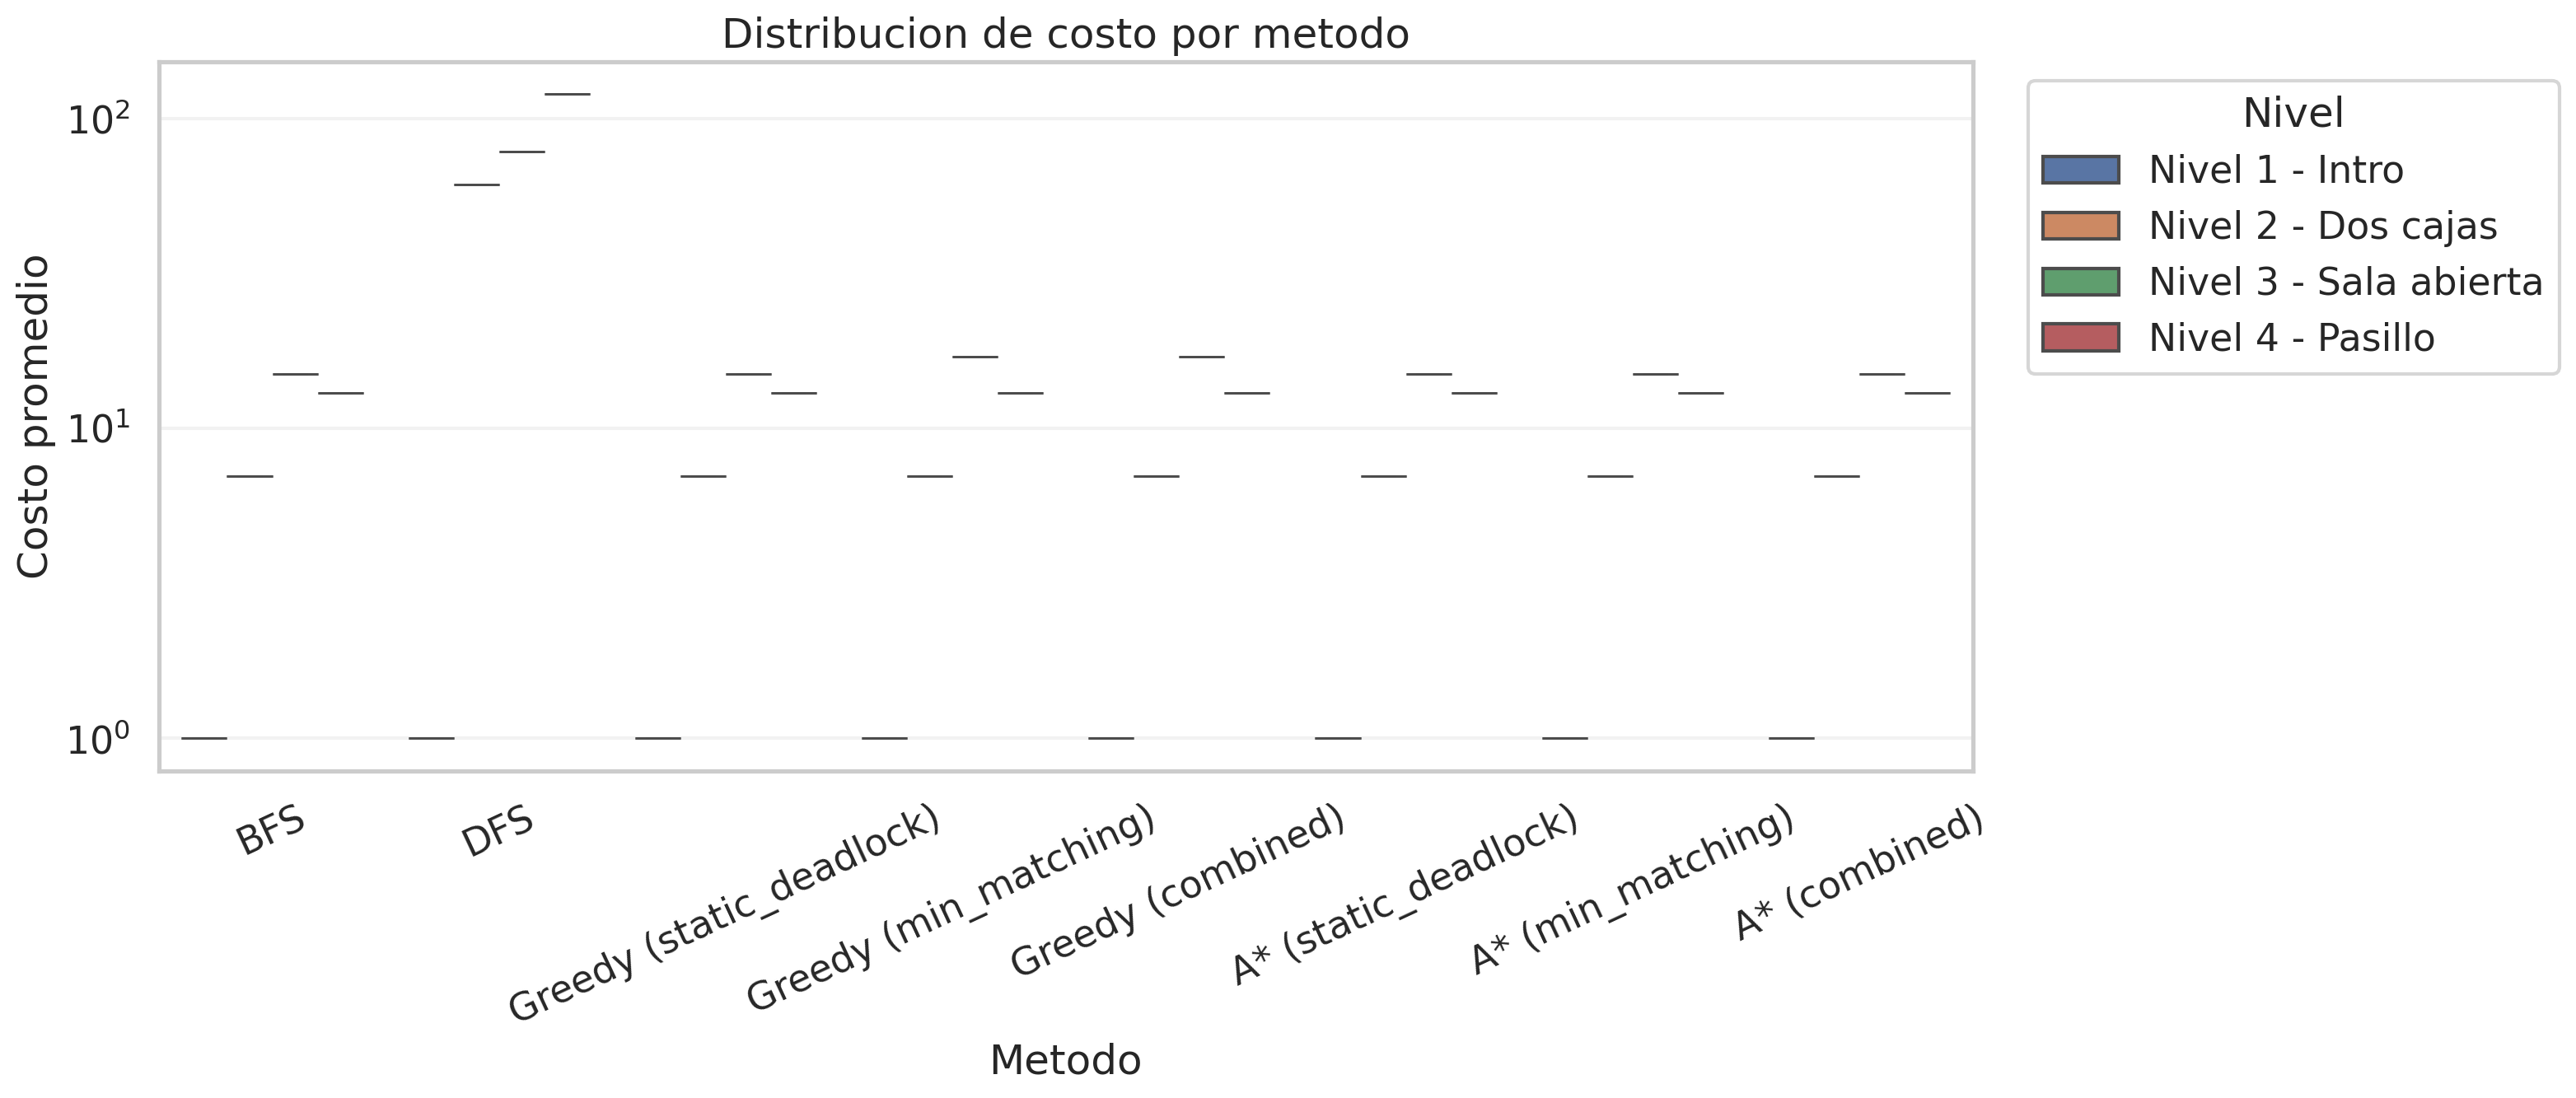
\includegraphics[width=0.85\textwidth]{../results/plots/boxplot_cost.png}
\caption{Distribucion de costo por metodo. Las cajas son planas porque la busqueda es determinista (los nodos expandidos, frontera y costo no varian entre iteraciones; solo el tiempo fluctua por ruido del OS).}
\end{figure}

% =============================================================================
\section{Analisis}
% =============================================================================

\subsection{Optimalidad}

BFS y todas las variantes de A* encuentran la solucion optima en todos los niveles. DFS encuentra soluciones hasta 9$\times$ mas largas que el optimo (120 vs 13 en Nivel 4). Greedy con min\_matching empata el optimo en 3 de 4 niveles pero no lo garantiza (en Nivel 3 da costo 17 vs optimo 15).

\subsection{Eficiencia de las heuristicas}

La heuristica de \textbf{min\_matching} es significativamente mas informativa que \textbf{static\_deadlock}:

\begin{itemize}
  \item A*(min\_matching) expande 133 nodos en Nivel 3 vs 680 de A*(static\_deadlock) --- 5$\times$ menos.
  \item La razon: static\_deadlock devuelve $h=0$ para estados no muertos, funcionando como test de poda binario pero sin guiar la busqueda. min\_matching da informacion numerica de cuanto falta.
  \item La combinada (combined) no aporta mejora sobre min\_matching sola en estos niveles, porque min\_matching ya es consistente y no hay reaperturas.
\end{itemize}

\subsection{Rol de static\_deadlock}

Aunque static\_deadlock aporta poco como heuristica numerica, su rol como \textbf{mecanismo de poda} es valioso: en niveles con posibilidades de deadlock, descarta ramas enteras devolviendo $\infty$. Esto explica por que A*(static\_deadlock) expande menos que BFS pese a tener $h=0$ para la mayoria de estados.

\subsection{Determinismo de las iteraciones}

La busqueda es completamente determinista (orden fijo de sucesores, semillas fijas). Las 10 iteraciones producen exactamente los mismos nodos expandidos, frontera y costo. Solo el tiempo de ejecucion varia por ruido del sistema operativo. Las barras de error en metricas distintas al tiempo son de ancho cero.

% =============================================================================
\section{Metricas reportadas}
% =============================================================================

Al finalizar cada corrida se reporta:

\begin{enumerate}
  \item \textbf{Resultado}: exito o fracaso.
  \item \textbf{Costo de la solucion}: cantidad de acciones del plan (cada movimiento del jugador cuesta 1).
  \item \textbf{Nodos expandidos}: estados sacados de la frontera y cuyos sucesores fueron generados.
  \item \textbf{Nodos frontera}: tamano de la frontera al momento de terminar la busqueda.
  \item \textbf{Solucion}: secuencia de acciones (UP, DOWN, LEFT, RIGHT) desde el estado inicial al goal.
  \item \textbf{Tiempo de procesamiento}: medido con \texttt{time.perf\_counter()}.
\end{enumerate}

Adicionalmente, para A*, se reportan metricas de diagnostico: \texttt{stale\_skipped} (entradas obsoletas en el heap), \texttt{reopened\_states} (nodos cerrados reabiertos) y \texttt{heuristic\_cache\_hits}.

% =============================================================================
\section{Tests}
% =============================================================================

El proyecto incluye 36 tests unitarios distribuidos en 7 archivos:

\begin{itemize}
  \item \textbf{test\_search\_astar.py} (5 tests): reapertura de nodos, entradas stale, tie-breaking, cache de heuristica, politica de deadlocks.
  \item \textbf{test\_search\_algorithms.py} (6 tests): DFS encuentra solucion, Greedy encuentra solucion, Greedy $\geq$ BFS en costo, estado ya resuelto retorna costo 0, roundtrip de render, guard de recursion.
  \item \textbf{test\_min\_matching.py} (9 tests): cajas en goals, una caja, matching optimo vs greedy, admisibilidad, combinada, A* iguala BFS en costo.
  \item \textbf{test\_static\_deadlocks.py} (8 tests): goals no prohibidos, esquinas prohibidas, BFS inverso, poda de sucesores, heuristica infinito, combinada, cache.
  \item \textbf{test\_level\_io.py} (3 tests): tableros irregulares, validacion de entidades, carga de archivos.
  \item \textbf{test\_deadlock\_policy.py} (2 tests): flags CLI, forwarding de politica.
  \item \textbf{test\_benchmark\_script.py} (2 tests): parsing de specs, forwarding por entrada.
  \item \textbf{test\_experiment\_runner.py} (1 test): pipeline completo genera outputs esperados.
\end{itemize}

% =============================================================================
\section{Conclusiones}
% =============================================================================

\begin{enumerate}
  \item \textbf{Las heuristicas informadas reducen drasticamente la exploracion.} A*(min\_matching) expande 31$\times$ menos nodos que BFS en el nivel con mayor branching.

  \item \textbf{No todas las heuristicas son iguales.} static\_deadlock es una poda binaria ($0$ o $\infty$) util para descartar estados imposibles, pero no guia la busqueda. min\_matching da informacion numerica que ordena eficientemente la frontera.

  \item \textbf{La combinacion con max es segura.} $\max(h_1, h_2)$ preserva admisibilidad y aprovecha ambas senales. En estos niveles, combined no mejora sobre min\_matching sola, pero en niveles mas grandes con deadlocks la poda seria mas valiosa.

  \item \textbf{A* con reapertura garantiza optimalidad con heuristicas admisibles.} La implementacion reabre nodos cerrados cuando encuentra un camino mas barato, eliminando la necesidad de consistencia para la garantia de optimalidad.

  \item \textbf{DFS no es adecuado para Sokoban.} Encuentra soluciones hasta 9$\times$ mas largas que el optimo, con el mayor numero de nodos expandidos.

  \item \textbf{Greedy es un buen compromiso practico.} Con min\_matching, empata o se acerca al optimo en estos niveles y explora una fraccion minima del espacio. Pero no garantiza optimalidad.
\end{enumerate}

\end{document}
